\section{Experiments}
% \label{sec:experiments}

%%% SECTION %%%
\subsection{Architectural hyper-parameters}
\label{sec:arch_hyper_params}
The backbone \emph{Temporal} Transformer of \ours{} has a latent dimension of 2048 (8192 for the SiLU gating), 28 layers, 16 heads and local attention over 3000 tokens, \emph{i.e.}, 2B parameters and a 4min context. The \emph{Depth} Transformer has a latent dimension of 1024 (4096 for the gating), 6 layers per codebook and 16 heads. It models $Q=16$ audio codebooks for the output stream and the same for the input stream but only at training. We reduce the size of the model before RL by distillation into a smaller one using weight sharing among the codebooks of the \emph{Depth} Transformer. Our final model architecture contains 3B parameters.

\begin{table*}[t]
    \caption{Objective comparison of \ours{} with Seamless~\citep{seamless} and Hibiki~\citep{hibiki} on short-form (Europarl-ST) and long-form (Audio-NTREX-4L) test data introduced in Section~\ref{sec:eval_datasets}.}
    \label{tab:objective_results}
    % \vskip 0.15in
    \begin{center}
    \begin{sc}
    \resizebox{0.975 \linewidth}{!}{%
    \begin{tabular}{lcccccccccccc}
    \toprule
     & \multicolumn{6}{c}{Short-form} & \multicolumn{6}{c}{Long-form} \\
    \cmidrule(lr){2-7}\cmidrule(lr){8-13}
          &                   & ASR               & ASR & Speaker           & End & & & ASR & ASR & Speaker & End & \\
    & BLEU ($\uparrow$) & BLEU ($\uparrow$) & COMET ($\uparrow$) & Sim. ($\uparrow$) & Offset ($\downarrow$) & LAAL ($\downarrow$) & BLEU ($\uparrow$) & BLEU ($\uparrow$) & COMET ($\uparrow$) & Sim. ($\uparrow$) & Offset ($\downarrow$)  & LAAL ($\downarrow$) \\
    \midrule
    \textbf{Seamless} \\
    French
        & 33.8 & 32.8 & 76.6 & 19.1 & 2.4 & \textbf{2.8}
        & 27.8 & 23.9 & 33.7 & 44.4 & 3.2 & 6.2 \\
    Spanish
        & \textbf{34.4} & 33.6 & 79.1 & 21.9 & 2.6 & 2.7
        & 29.9 & 25.2 & 36.1 & 42.6 & 2.8 & 6.5 \\
    Portuguese
        & \textbf{34.1} & \textbf{33.6} & 78.9 & 23.9 & 2.8 & 3.1
        & 29.0 & 25.6 & 35.0 & 35.7 & 3.2 & 6.6 \\
    German
        & 27.8 & 27.3 & \textbf{82.3} & 20.6 & 2.4 & 3.0
        & 27.8 & 24.0 & 40.6 & 47.8 & 2.5 & 7.3 \\
    \midrule
    \textbf{Hibiki} \\
    French
        & 32.4 & 31.8 & \textbf{81.5} & 35.7 & 2.5 & 3.5
        & 29.5 & 26.4 & 42.0 & 52.8 & 2.6 & 6.8 \\  %
    \midrule
    \textbf{\ours{}} \\  % DISTIL 77f82164@110
    French
        & \textbf{35.0} & \textbf{34.6} & 80.3 & \textbf{49.5} & \textbf{2.1} & \textbf{2.8}
        & \textbf{30.6} & \textbf{28.7} & \textbf{43.7} & \textbf{61.3} & \textbf{2.3} & \textbf{6.1} \\
    Spanish
        & 33.8 & \textbf{33.9} & \textbf{80.3} & \textbf{57.0} & \textbf{2.3} & 3.1
        & \textbf{32.3} & \textbf{31.5} & \textbf{42.3} & \textbf{64.6} & \textbf{2.6} & \textbf{5.6} \\
    Portuguese
        & 33.6 & \textbf{33.6} & \textbf{78.9} & \textbf{51.4} & \textbf{2.4} & \textbf{3.0}
        & \textbf{33.2} & \textbf{31.3} & \textbf{42.6} & \textbf{62.1} & \textbf{2.3} & \textbf{6.3} \\
    German
        & \textbf{28.7} & \textbf{28.6} & 82.0 & \textbf{51.5} & \textbf{1.9} & \textbf{2.8}
        & \textbf{29.1} & \textbf{28.3} & \textbf{42.3} & \textbf{66.0} & \textbf{2.0} & \textbf{5.9} \\
    \bottomrule
    \end{tabular}}
    \end{sc}
    \end{center}
    % \vskip -0.1in
\end{table*}

%%% SECTION %%%
\subsection{Training protocol}
\label{sec:training_protocol}
We train a multilingual-to-English speech translation system through the following steps, each with a cosine learning rate schedule and AdamW~\citep{adamw}, with weight decay of 0.1, and momentum parameters (0.9, 0.95).

\subsubsection{Text backbone initialization}
\label{sec:text_pretraining}
We initialize the \emph{Temporal} Transformer with Helium-1\footnote{\href{https://huggingface.co/kyutai/helium-1-2b}{huggingface.co/kyutai/helium-1-2b}} \citep{helium} weights, an open-source base text LLM with 2B parameters trained using filtered Common Crawl\footnote{\href{https://commoncrawl.org}{commoncrawl.org}} data.

\subsubsection{Audio pretraining}
\label{sec:audio_pretraining}
Starting from the pretrained text backbone, weights of the \emph{Depth} Transformer are added to the architecture as well as audio tokens projection layers. We perform an audio pretraining with single stream audio as done by \citet{hibiki} but on multilingual speech. Our data mixture comprises approximately 12\% of audio in each input language, 50\% of English and less than 2\% of Italian. We train for 1K steps with a batch size of 144 and a learning rate of $2\cdot10^{-4}$. After this pretraining stage, we duplicate the weights of the \emph{Depth} Transformer to allow for future multistream training.

\subsubsection{Coarse speech translation training}
\label{sec:st_training}

We construct a large-scale multilingual-to-English speech translation dataset comprising $40,000$ hours for each source language (French, Spanish, Portuguese, and German). Starting from a massive collection of multilingual audio, we extract 4 million single-speaker utterances, whose durations are between 30 and 75 seconds, and transcribe them using Whisper large-v3~\citep{whisper}. Transcripts are partitioned into sentences via Spacy's \texttt{core\_news\_sm} and individually translated using MADLAD-3B~\citep{madlad}, after which we synthesize the target speech using the TTS system described in Section~\ref{sec:nat_pauses_tts} with 10-second speaker conditioning. To ensure coarse translation alignments, we apply the silence insertion technique from Section~\ref{sec:sent_level_align} using $\delta=0.5$ and $\mu=2$. Scaling our training budget following \citet{hibiki}, we perform $500,000$ gradient steps with a batch size of 96 and a learning rate of $3\cdot10^{-5}$, computing the loss on both source and target streams with source noise augmentation. Finally, sequence termination is explicitly modeled by inserting a special input EOS token immediately following the source utterance and a separate EOS token in the text stream to demarcate the end of generation. Appendix Table~\ref{tab:multi_vs_monolingual} compares the performance of multilingual and monolingual models.

\subsubsection{Speech translation fine-tuning}
\label{sec:st_finetuning}
We use the synthetic data generation method with natural pauses introduced in Section~\ref{sec:nat_pauses_tts} to build a synthetic multilingual speech translation dataset of less than 200h in total. We fine-tune for 1K steps with a batch size of 16, a learning rate of $1\cdot10^{-6}$ and other configurations being similar to the previous phase described in \ref{sec:st_training}. We then distill the model into a light copy of itself with codebooks weight sharing using the same dataset and 20K gradient updates.

\subsubsection{Reinforcement learning}
\label{sec:st_rl}
Starting from the light fine-tuned translation model, we use data from the speech translation training introduced in Section~\ref{sec:st_training} and run our reinforcement learning process as described in Section~\ref{sec:rl_method}. We train with a batch size of 32, a group size of 4, learning rate of $2\cdot10^{-7}$ and perform 2000 updates with $\tau=20$. Sequences of length $T=1500$ frames are generated using a temperature of 0.8 and top-k of 250 for both text and audio streams. Process rewards are computed every $n_w=8$ input words and we set $\alpha=0.4$ and $\epsilon=0.2$. We use $c_0=100$ and $c_q=1$ for $q \ge 1$ to balance loss between text and audio streams. The model is evaluated every $10\cdot\tau$ updates on a valid set and we define Hibiki-Zero as the checkpoint with the best quality/latency trade-off according to objective evaluation metrics. Appendix Table~\ref{tab:base_and_finetuned_results} compares our base and fine-tuned models to \ours{}.

%%% SECTION %%%
\subsection{Evaluation datasets}
\label{sec:eval_datasets}

\paragraph{Long-form data.}
We build Audio-NTREX-4L, a multilingual long-form ST dataset using text translations from the NTREX~\cite{ntrex} corpus. We select 300 examples for each source language and synthesize them using the following high-quality TTS from the industry: ElevenLabs\footnote{\href{https://elevenlabs.io/text-to-speech}{elevenlabs.io/text-to-speech} (``eleven-multilingual-v2 TTS'')}, Cartesia\footnote{\href{https://cartesia.ai/sonic}{cartesia.ai/sonic} (``sonic-v2 TTS'')} and Gradium\footnote{\href{https://gradium.ai/\#models}{gradium.ai/\#models} (``default TTS'')}. We condition generations using voices from the multilingual dataset CML-TTS~\citep{cml_tts}. Audio-NTREX-4L contains around 15h of speech per TTS with an average duration of 45 seconds per sample and is split in balanced valid and test sets.
% \footnote{\href{https://www.openslr.org/146/}{openslr.org/146/}}

\paragraph{Short-form data.}
We filter data from Europarl-ST~\citep{europarl_st} and retain samples with realistic transcripts and duration between 2 and 20 seconds. We build valid and test sets, each with 1024 samples per source language for a total of 10h hours per set.
% \footnote{\href{https://mllp.upv.es/europarl-st/}{mllp.upv.es/europarl-st/}}


%%% SECTION %%%
\subsection{Evaluation metrics}
\label{sec:eval_metrics}

\looseness=-1
\paragraph{Translation quality.} We evaluate translation quality by transcribing generated speech using Whisper medium~\cite{whisper} and computing BLEU~\cite{sacrebleu} and COMET~\cite{comet} scores with respect to a reference translation, referred to as ASR-BLEU and ASR-COMET. To reduce the impact of ASR errors, hypothesis and reference texts are normalized\footnote{\href{https://github.com/openai/whisper/blob/main/whisper/normalizers/english.py}{github.com/openai/whisper/blob/main/whisper/normalizers}} before computing BLEU scores. Since Seamless and \ours{} perform speech-to-text translation in parallel, we also compute BLEU and COMET scores using their text outputs. We use the XCOMET-XL model.\footnote{\href{https://github.com/Unbabel/COMET}{github.com/Unbabel/COMET}}.

\looseness=-1
\paragraph{Translation Latency.} We rely on two common latency metrics known as End Offset and LAAL (Length-Adaptive Average Lagging). End Offset is defined as the time difference (in seconds) between the end of the last generated word and the end of the last word from the source. We compute LAAL following the method described by \citet{laal} which defines it as an approximation of the average time (in seconds) between a source word and its translation. We use word-level emission timestamps $(d_i)_{1 \dots n_{\mathrm{gen}}}$ produced by Whisper for $n_{\mathrm{gen}}$ words in the generated speech. We define $\gamma = \frac{\Delta_{\mathrm{source}}}{\max(n_{\mathrm{gen}}, n_{\mathrm{ref}})}$ where $\Delta_{\mathrm{source}}$ is the duration of the source speech and $n_{\mathrm{ref}}$ the number of words in the reference translation. The LAAL score is then computed as $\frac{1}{n_{\mathrm{max}}}\sum_{i=1}^{n_{\mathrm{max}}} d_i - (i-1)\gamma$ where $n_{\mathrm{max}} = \mathrm{min}\{i|d_i \geq \Delta_{\mathrm{source}}\}$.

\begin{table}[t]
    \caption{\textbf{Human evaluation.} Raters report Mean Opinion Scores (MOS) on a scale ranging from 0 to 100 for each audio sample.}
    \label{tab:human_eval}
    \begin{center}
    \begin{scriptsize}
    \begin{sc}
    \begin{tabular}{@{}ll@{\hspace{5pt}}c@{\hspace{5pt}}c@{\hspace{5pt}}c@{}}
    \toprule
    Input    & \multirow{2}{*}{Model} & Audio   & Speaker    & Speech \\
    language &                        & Quality & Similarity & Naturalness \\
    \midrule
    \multirow{3}{*}{French} & Seamless & 11.4 $\pm$ 3.1 & 21.1 $\pm$ 4.9 & 21.2 $\pm$ 3.8 \\
                            & Hibiki & 62.9 $\pm$ 4.8 & 44.7 $\pm$ 5.1 & 57.0 $\pm$ 4.2 \\
                            & \ours{} & \textbf{64.5} $\pm$ 4.2 & \textbf{70.0} $\pm$ 5.1 & \textbf{67.2} $\pm$ 4.1 \\
    \midrule
    \multirow{2}{*}{Spanish} & Seamless & 10.7 $\pm$ 2.6 & 21.2 $\pm$ 4.5 & 26.5 $\pm$ 4.4 \\
                             & \ours{} & \textbf{66.8} $\pm$ 3.9 & \textbf{69.0} $\pm$ 3.9 & \textbf{66.2} $\pm$ 4.9 \\
    \midrule
    \multirow{2}{*}{Portuguese} & Seamless & 11.8 $\pm$ 3.1 & 32.5 $\pm$ 6.0 & 22.8 $\pm$ 3.9 \\
                                & \ours{} & \textbf{62.0} $\pm$ 4.1 & \textbf{60.7} $\pm$ 4.2 & \textbf{75.6} $\pm$ 3.4 \\
    \midrule
    \multirow{2}{*}{German} & Seamless & 15.6 $\pm$ 2.7 & 25.2 $\pm$ 4.9 & 26.4 $\pm$ 4.8 \\
                            & \ours{} & \textbf{73.5} $\pm$ 3.4 & \textbf{65.3} $\pm$ 4.3 & \textbf{69.9} $\pm$ 3.9 \\
    \bottomrule
    \end{tabular}
    \end{sc}
    \end{scriptsize}
    \end{center}
\end{table}

\begin{table}[t]
    \caption{Objective results of model adaptation to input Italian speech with 850 hours of finetuning data on short-form evaluation.}
    \label{tab:italian_results}
    \begin{center}
    \setlength{\tabcolsep}{3pt}
    \begin{scriptsize}
    \begin{sc}
    \begin{tabular}{lccccc}
    \toprule
    & BLEU                  & ASR               & Speaker           & End                   & LAAL \\
    &          ($\uparrow$) & BLEU ($\uparrow$) & Sim. ($\uparrow$) & Offset ($\downarrow$) & ($\downarrow$) \\
    \midrule
    \textbf{Seamless} & \textbf{32.5} & \textbf{32.0} & 22.2 & \textbf{3.0} & \textbf{3.5} \\
    \midrule
    \textbf{Ours} \\
    Base & 14.3 & 14.3 & 50.6 & 3.9 & 4.3 \\  % 5c94ad8f@500
    Finetuned & 31.4 & 31.0 & \textbf{55.2} & 3.7 & 4.5 \\  % 6f8df93b@200
    Finetuned + RL & 32.1 & 31.9 & 54.2 & \textbf{3.0} & \textbf{3.5} \\  % a475c272@100
    \bottomrule
    \end{tabular}
    \end{sc}
    \end{scriptsize}
    \end{center}
\end{table}

\looseness=-1
\paragraph{Cross-lingual speaker similarity.} For objective voice transfer evaluation, we use a standard model for speaker verification\footnote{\href{https://github.com/microsoft/UniSpeech/tree/main/downstreams/speaker\_verification\#pre-trained-models}{github.com/microsoft/UniSpeech} (``WavLM Large'')} based on WavLM~\cite{wavlm} and report the cosine similarity between the embeddings of the source and the generated speech.

\looseness=-1
\paragraph{Audio quality and naturalness.} We rely on human raters to evaluate audio quality, speech naturalness and additional cross-lingual speaker similarity of generated audios. We conduct evaluations per input language using 50 samples and 20 raters for each model with 5 comparisons per rater.
% The detailed protocol is given in Appendix.

%%% SECTION %%%
\subsection{Inference configuration}
\label{inference_config}
We encode audio with the streaming codec and feed the tokens to \ours{} while decoding the output tokens to obtain a streaming translation. At the end of the input, we force EOS tokens to our model input audio streams, and keep sampling until it produces its own text stream EOS. We use temperature of 0.8 and top-k of 250 for all tokens.

%%% SECTION %%%
\subsection{Results}

\paragraph{Objective evaluations.}
\label{sec:objective_st_results}
Table~\ref{tab:objective_results} compares \ours{} against the best available baselines for simultaneous S2ST namely Seamless~\citep{seamless} and Hibiki~\citep{hibiki} with the latter only supporting French as input. Our model outperforms both baselines on long-form speech translation with more than 5pts of ASR BLEU, 20pts of speaker similarity and lower latency compared to Seamless. In the short-form setting, our approach outperforms Hibiki by 3pts of ASR BLEU while being faster and is on par with Seamless on the quality/latency trade-off but surpasses it on speaker similarity by more than 30pts.

\paragraph{Audio fidelity and speech expressivity.}
\label{sec:human_eval_results}
Human evaluations reported in Table~\ref{tab:human_eval} confirm the clear advantage of \ours{} compared to Seamless on speaker identity transfer but also show that it produces higher quality audio with better speech naturalness. Compared to Hibiki on a French-to-English task, our model reaches equivalent audio quality while being more natural with a better speaker similarity.

\paragraph{New language adaptation.}
\label{sec:new_lang_results}
Following our method from Section~\ref{sec:st_training}, we build a small coarse-aligned Italian-to-English ST dataset containing less than 1000 hours in each language. Starting from the base translation model obtained after the training stage described in Section~\ref{sec:st_training}, we fine-tune and apply our RL method for the Italian-to-English translation task only. Results are presented in Table~\ref{tab:italian_results} and show that we attain the same translation quality/latency trade-off as Seamless with better speaker similarity on an extension to Italian of our short-form evaluation data. As shown in Appendix Table~\ref{tab:italian_results_longform}, our model adapted to Italian also retains most of its capabilities on the original languages.


%%% SECTION %%%
\subsection{Ablations}
\label{sec:ablations}

We present ablation results in figures~\ref{fig:ablation_alpha}, \ref{fig:ablation_fw} and \ref{fig:ablation_misc_setup} using exponential moving average smoothing for readability. Performance during RL is represented using BLEU and text LAAL metrics. They are computed every $\tau$ updates on a validation set using the output text stream of the model which is synchronized with the output audio. As observed by~\citet{hibiki}, we also notice very high BLEU scores (around 60) compared to evaluation scores (around 30). Indeed, our train and valid sets were obtained with the same data generation process described in Section~\ref{sec:st_training} thus following the same translation style as MADLAD-3B~\citep{madlad} that our ST models learn to replicate.

\paragraph{Ablation: Quality/Latency control during RL.}
\label{sec:ablation_alpha}
We benchmark the effect of parameter $\alpha$ introduced in Section~\ref{sec:process_rewards} which balances total and intermediate BLEU scores in the definition of process rewards. As illustrated in Figure~\ref{fig:ablation_alpha}, performing RL with high values of $\alpha$ leads to a higher translation latency but better overall translation quality as expected. On the contrary, lower values of $\alpha$ reduce latency further at the cost of a limited quality decrease.

\paragraph{Ablation: Process rewards computation frequency.}
\label{sec:ablation_fw}
Using $\alpha=0.5$, we study the effect of parameter $n_w$ introduced in Section~\ref{sec:optim_objective} which controls how often process rewards are computed along a generated sequence. As shown in Figure~\ref{fig:ablation_fw}, decreasing this parameter below $8$ does not significantly impact the final quality/latency trade-off.

\begin{figure}[t]
    \centering
    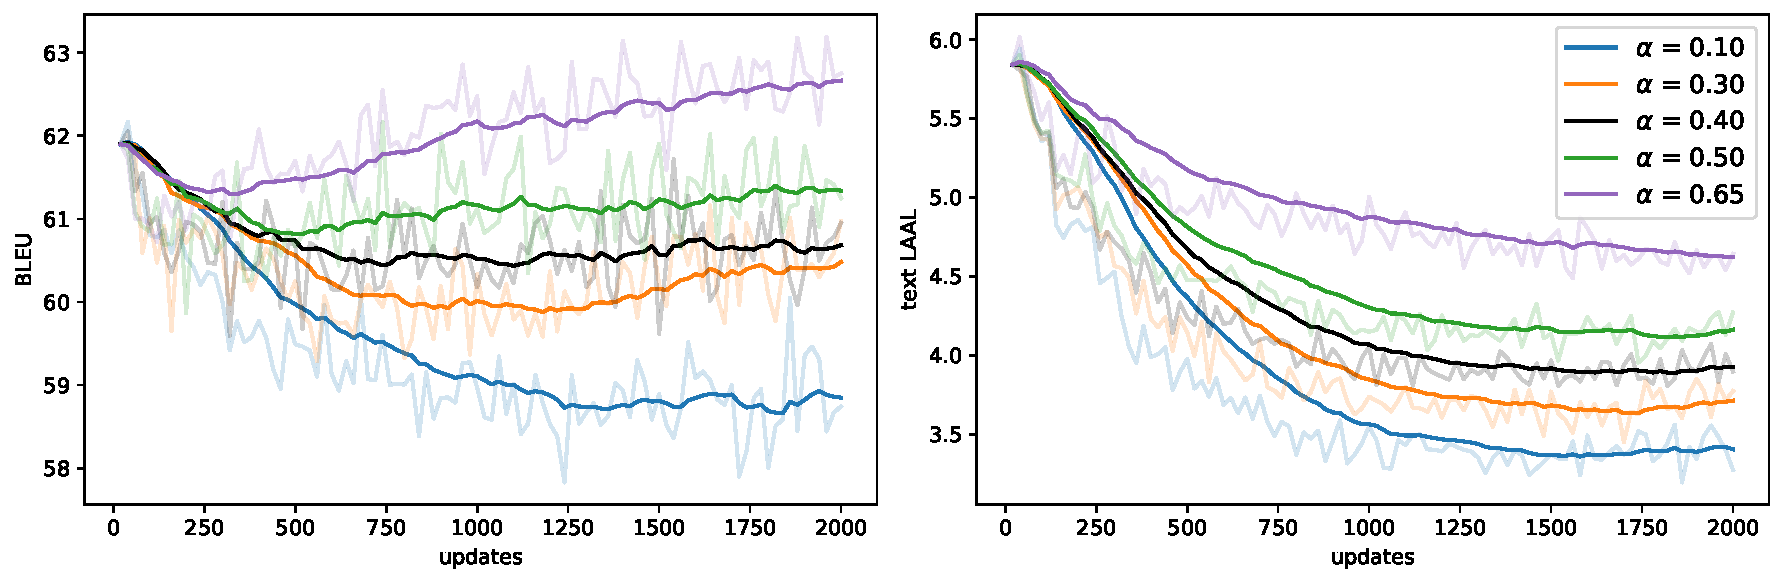
\includegraphics[width=\columnwidth]{figures/ablation_alpha_curves.pdf}
    \caption{\textbf{Influence of hyperparameter $\alpha$ during RL.} We plot the BLEU score and text LAAL over training for various $\alpha$ (see Eq.~\eqref{eq:process_reward}), starting from the same supervised model using $n_w=8$.}
    \label{fig:ablation_alpha}
\end{figure}

\begin{figure}[t]
    \centering
    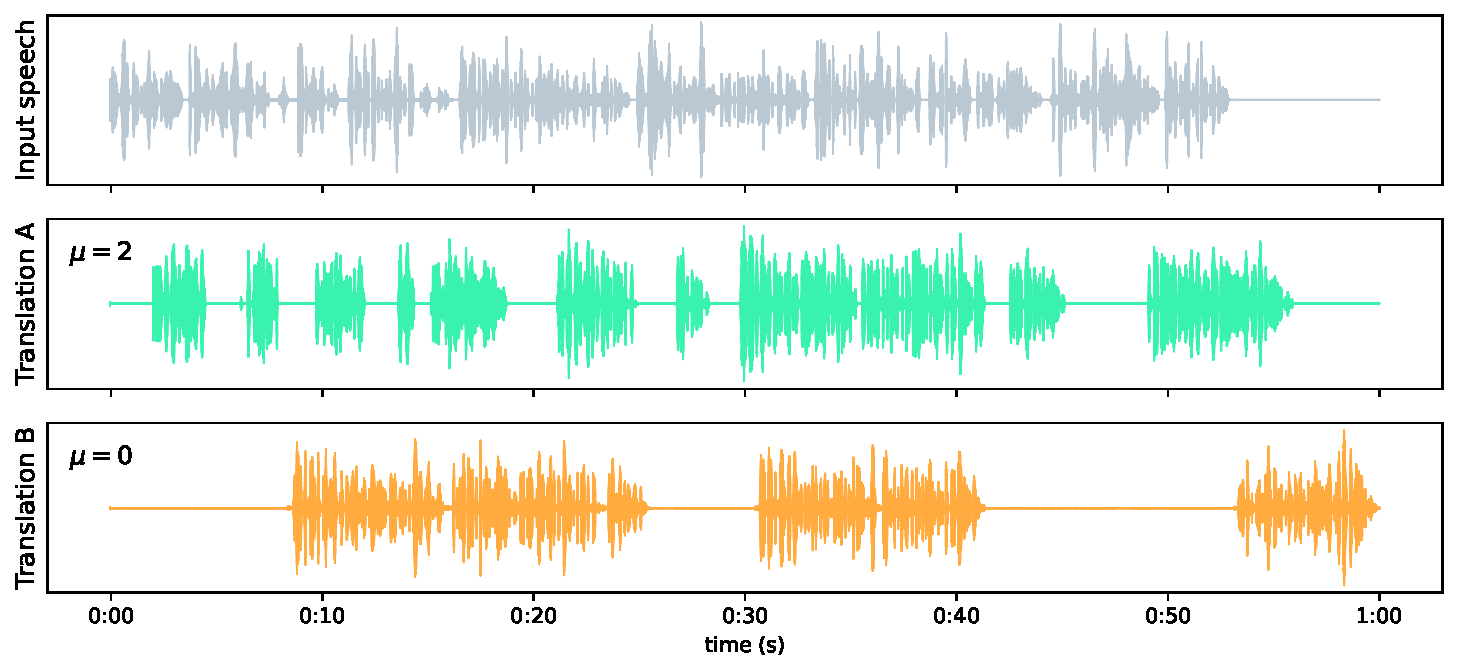
\includegraphics[width=\columnwidth]{figures/baseline_silences_patterns.pdf}
    \caption{\textbf{Illustration of coarse translation alignment patterns} Waveform A is generated by a model trained on coarse alignments with random silences. Waveform B is generated by a model trained on coarse alignments with silences between sentences only.}
    \label{fig:baseline_silences_pattern}
\end{figure}

\begin{figure}[t]
    \centering
    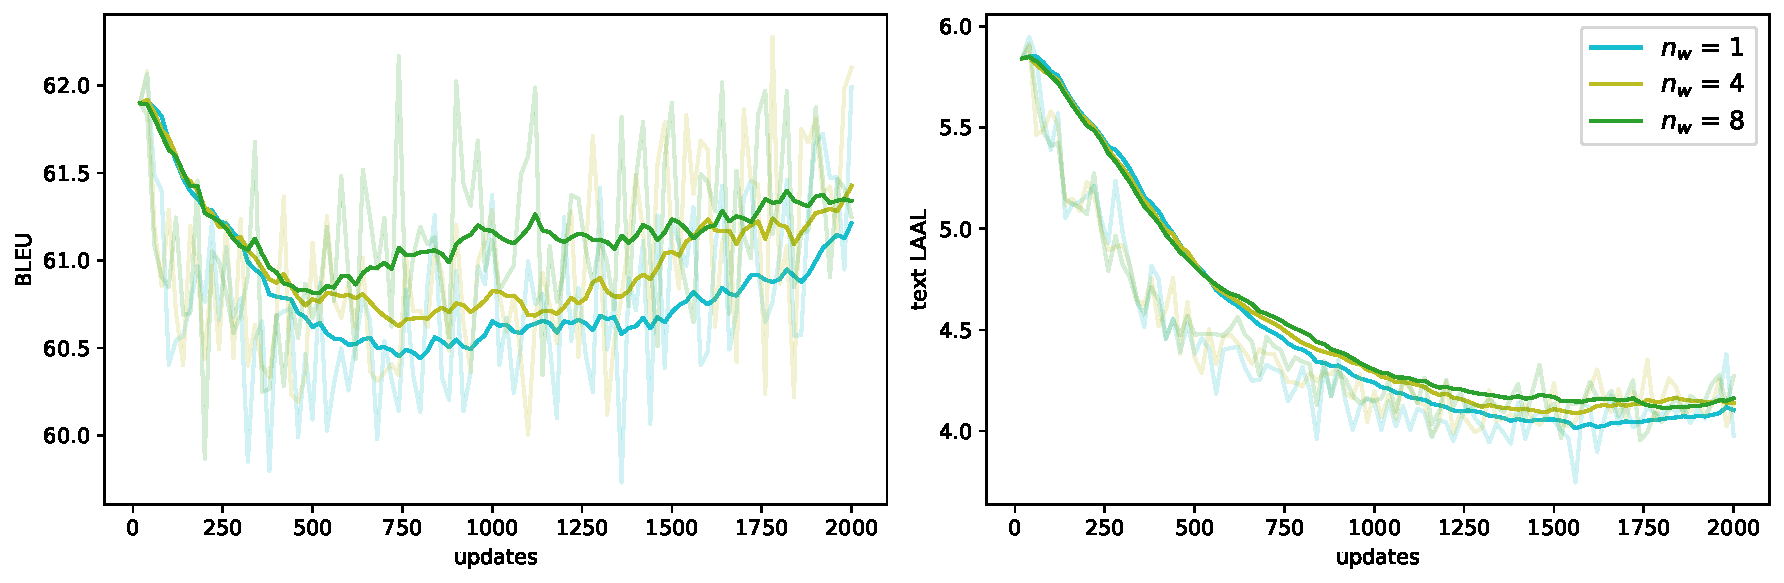
\includegraphics[width=\columnwidth]{figures/ablation_fw_curves.pdf}
    \caption{\textbf{Influence of hyperparameter $n_w$ during RL.} We plot the BLEU score and text LAAL over training for various $n_w$ (see Sec.~\ref{sec:optim_objective}) starting from the same supervised model using $\alpha=0.5$.}
    \label{fig:ablation_fw}
\end{figure}

\begin{figure}[t]
    \centering
    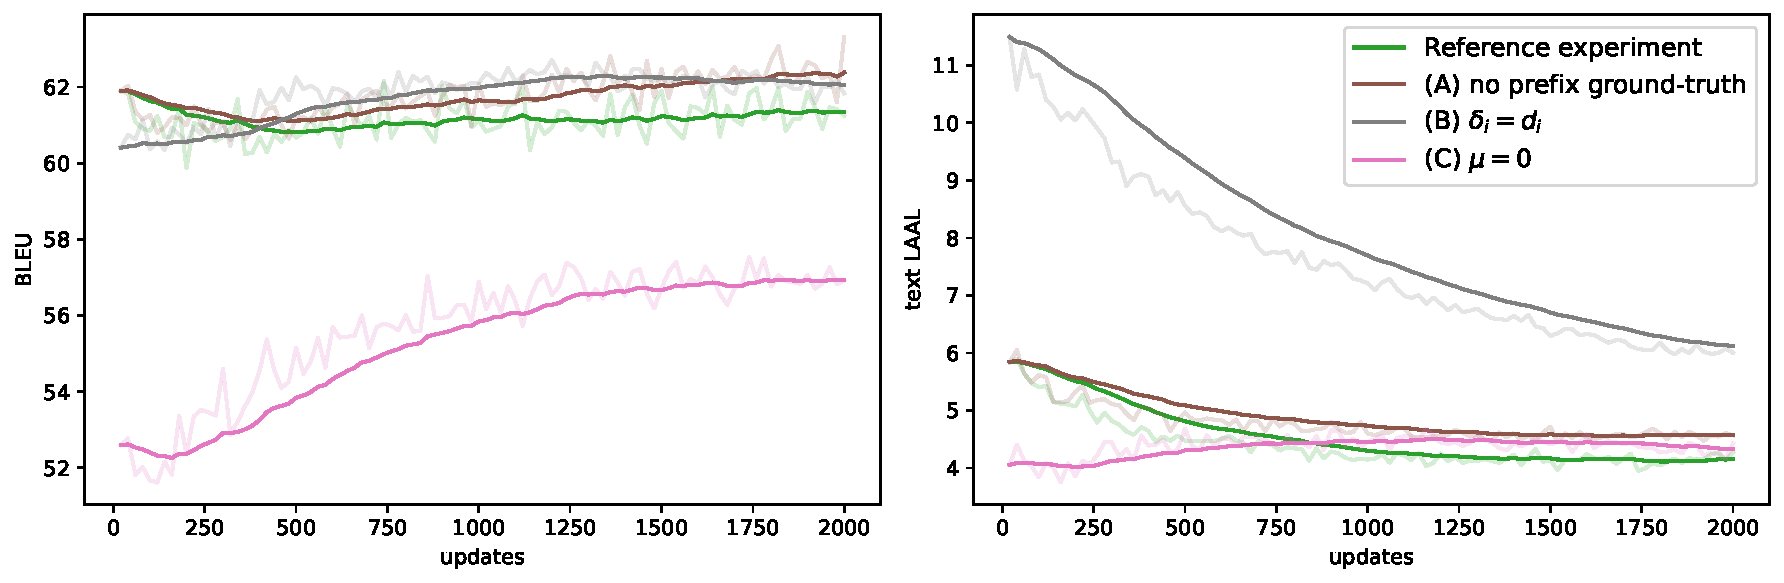
\includegraphics[width=\columnwidth]{figures/ablation_misc_setup_curves.pdf}
    \caption{\textbf{Alternative configurations.} We use $\alpha=0.5$ and $n_w=8$ for all experiments. Experiment (A) uses the full translation of the input speech as reference to compute process rewards instead of sentence-level prefixes as in Equation~\ref{eq:process_reward}. Experiment (B) performs RL on a supervised model trained with full sentence-delay i.e. $\delta_i=d_i$ for each input sentence of index $i$. Experiment (C) performs RL on a supervised model trained with coarse alignments using silences between sentences only i.e. $\mu=0$.}
    \label{fig:ablation_misc_setup}
\end{figure}

\paragraph{Ablation: Alternative configurations.}
\label{sec:ablation_misc}

In Figure~\ref{fig:ablation_misc_setup}, we compare alternative configurations that could be used for model development instead of our main setup referred to as \textit{Reference experiment}. We keep $\alpha=0.5$ and $n_w=8$ fixed. \\

Experiment (A) performs RL using the full translation of the reference input text instead of sentence-level prefixes to compute intermediate BLEU scores. This amounts to modify Equation~\ref{eq:process_reward} so it becomes $r^{(i)}_{\mathrm{noprefix},t} = (1 - \alpha) \mathrm{BLEU} ( \hat{y}^{(i)}_{t}, y_{T} ) + \alpha \mathrm{BLEU} ( \hat{y}^{(i)}_{T}, y_{T} )$. We observe better quality performance but at the cost of latency. According to us, this comes from intermediate BLEU scores being much noisier as translated references are too optimistic, making it harder to discriminate between sequences to optimize latency during RL. \\

Experiment (B) performs RL starting from a base model trained with full sentence delays between input and output speech meaning that $\delta_i=d_i$ for each sentence index $i$ using notations from Section~\ref{sec:sent_level_align}. Therefore, latency is much higher when starting RL and is reduced to around 6 seconds which remains far worse than the reference experiment. We also observe this behavior in preliminary experiments where RL was unable to teach the base model to start translation of an input sentence before it ends as the base model was never trained in that manner during supervised training. This justifies the use of $\delta_i<d_i$ when building coarse alignments so RL can benefit from exploration. \\

\vspace{-1em}
Experiment (C) performs RL starting from a base model trained with coarse alignments using sentence-level silences only ($\mu=0$). We observe a degradation both in terms of quality and latency compared to the reference experiment. The loss of quality is expected when decreasing $\mu$ as we don't delay as much the output with respect to the input. The cause of higher latency is illustrated in Figure~\ref{fig:baseline_silences_pattern} where waveform B ($\mu=0$) is a speech translation where silences are located between sentences only. This results in a higher average latency than waveform A ($\mu>0$) which presents a better distribution of speech along time.


%%% SECTION %%%
\subsection{Limitations}
\label{sec:limitations}

\looseness=-1
This work proposes an efficient method to perform multilingual speech translation and shows promising results on new input language adaptation.
However, while our model exhibits state-of-the-art speaker identity preservation, there is no way to control the intensity of the accent from the input language in the generated speech. Such control could be added by providing accent-annotated samples during supervised training and using conditioning at inference.